\documentclass[a4paper,11pt]{extarticle}

\usepackage[utf8]{inputenc} %кодировка
\usepackage[T1,T2A]{fontenc} % тоже кодировка
\usepackage[english,russian]{babel} %языки

\usepackage{multirow}
\usepackage{tabularx,booktabs}
\usepackage{floatrow}


\usepackage{graphicx, float} %пакет для единого оформления всех плавающих объектов (избегаем повторяющихся команд в документе)

\DeclareGraphicsExtensions{.pdf,.png,.jpg,.eps}%форматы
\usepackage{titlesec}
\setcounter{secnumdepth}{4}
\titleformat{\paragraph}
{\normalfont\normalsize\bfseries}{\theparagraph}{1em}{}
\titlespacing*{\paragraph}
{0pt}{3.25ex plus 1ex minus .2ex}{1.5ex plus .2ex}

\graphicspath{{images/}} % выбираем папку, в которую сохраняем все рисунки, чтобы не было хаоса файлов

\usepackage{amsmath,amssymb}%математические формулы и символы

\usepackage[a4paper,left=30mm,right=15mm,top=20mm,bottom=20mm]{geometry} % устанавливает поля документа

\parindent=4ex %красная строка
\parskip=5mm %расстояние между параграфами
\usepackage{indentfirst} %делать отступ в начале параграфа

\usepackage{hyperref} % добавление ссылок

\def\hmath$#1${\texorpdfstring{{\rmfamily\textit{#1}}}{#1}}
%настройка подписей плавающих объектов

\makeindex %нумерация

\usepackage{array,graphicx,caption} %картинки, подписи, таблицы
%\usepackage{endfloat} - для вывода картинок со списком в конце файла

\usepackage{caption} %подписи к картинкам

\usepackage[labelformat=simple]{subcaption} %для subfigure
\renewcommand\thesubfigure{(\alph{subfigure})}

\usepackage[export]{adjustbox} %чтобы влево-вправо картинки ставить

\usepackage[labelformat=simple]{subcaption}
% метка subfigure: "(а)" вместо дефолтного "а"

\renewcommand\thesubfigure{(\alph{subfigure})} % для продвинутого captionof

\usepackage{afterpage,placeins} % для барьеров

\usepackage{wrapfig} %добавление wrapfig

\usepackage[nottoc]{tocbibind} %подключает в содержание список лит-ры

\usepackage{multicol}

\usepackage{listings}

\usepackage[normalem]{ulem}
\usepackage{verbatim}
\usepackage[russian]{babel}

\usepackage{xcolor}

%New colors defined below
\definecolor{codegreen}{rgb}{0,0.6,0}
\definecolor{codegray}{rgb}{0.5,0.5,0.5}
\definecolor{codepurple}{rgb}{0.58,0,0.82}
\definecolor{backcolour}{rgb}{0.95,0.95,0.92}

%Code listing style named "mystyle"
\lstdefinestyle{mystyle}{
  backgroundcolor=\color{backcolour}, commentstyle=\color{codegreen},
  keywordstyle=\color{magenta},
  numberstyle=\tiny\color{codegray},
  stringstyle=\color{codepurple},
  basicstyle=\ttfamily\footnotesize,
  breakatwhitespace=false,
  breaklines=true,
  captionpos=b,
  keepspaces=true,
  numbers=left,
  numbersep=5pt,
  showspaces=false,
  showstringspaces=false,
  showtabs=false,
  tabsize=2
}

%"mystyle" code listing set
\lstset{style=mystyle}


\begin{document}

\begin{center}
МИНИСТЕРСТВО НАУКИ И ВЫСШЕГО ОБРАЗОВАНИЯ РОССИЙСКОЙ ФЕДЕРАЦИИ\\
\hfill \break
ФЕДЕРАЛЬНОЕ ГОСУДАРСТВЕННОЕ АВТОНОМНОЕ \\ ОБРАЗОВАТЕЛЬНОЕ УЧРЕЖДЕНИЕ ВЫСШЕГО ОБРАЗОВАНИЯ \\
“МОСКОВСКИЙ ФИЗИКО-ТЕХНИЧЕСКИЙ ИНСТИТУТ (НАЦИОНАЛЬНЫЙ ИССЛЕДОВАТЕЛЬСКИЙ УНИВЕРСИТЕТ)” \\

\hfill \break
Физтех-школа радиотехники и компьютерных технологий\\
\vspace{2.5cm}
\large{\textbf{Отчёт по лабораторной работе № 2.1.4}}\\
\large{\textbf{"Определение теплоемкости твердых тел"}}\\
\hfill \break
\end{center}

\vspace{5cm}

\begin{flushright}
Выполнил:\\
Студент гр. Б01-305\\
Миннахметов Артур\\
\end{flushright}

\vfill


\begin{center} Долгопрудный, 2024 \end{center}

\thispagestyle{empty}
\newpage


% \tableofcontents

% \newpage

\section{Введение}

\textbf{Цель работы:}
экспериментально исследовать свойства течения газов по тонким трубкам при различных числах Рейнольдса; выявить область применимости закона
Пуазейля и с его помощью определить коэффициент вязкости воздуха.

\textbf{В работе используются:}
система подачи воздуха (компрессор, поводящие трубки); газовый счетчик барабанного типа; спиртовой микроманометр с регулируемым
наклоном; набор трубок различного диаметра с выходами для подсоединения
микроманометра; секундомер.
\subsection{Теоритическая справка}
Работа посвящена изучению течения воздуха по прямой трубе круглого
сечения. Движение жидкости или газа вызывается перепадом внешнего
давления на концах $\Delta P$ трубы, чему в свою очередь препятствуют силы вязкого
(«внутреннего») трения, действующие между соседними слоями жидкости, а
также со стороны стенок трубы.

Сила вязкого трения как в жидкостях, так и в газах описывается законом
\textit{Ньютона}: касательное напряжение между слоями пропорционально перепаду
скорости течения в направлении, поперечном к потоку. В частности, если
жидкость течёт вдоль оси \textit{x}, а скорость течения $v_x(y)$ зависит от координаты \textit{y}, в
каждом слое возникает направленное по \textit{x} касательное напряжение
\begin{equation}
    \tau_{xy} = -\eta \frac{\partial v_x}{\partial y}.
\end{equation}

Характер течения определяется безразмерным параметром задачи -— числом Рейнольдса:
\begin{equation}
    \text{Re} = \frac{\rho ua}{\eta},
\end{equation}
где $u$ -- характерная скорость течения, $a$ -- характерный размер системы.

В целях упрощения теоретической модели течение газа в условиях
эксперимента можно считать несжимаемым, то есть принять плотность среды
постоянной: $\rho$ = const. Для газов такое приближение допустимо, если
относительный перепад давления в трубе мал $\Delta P\ll P $, а скорость течения
значительно меньше скорости звука (число Маха много меньше единицы). В нашем
опыте максимальная разность давлений составляет $\sim$ 30 см водного столба
(3 кПа), что составляет $\sim$ 3\% от атмосферного давления, причем в «рабочем»
(ламинарном) режиме перепад в несколько раз меньше ($\sim$ 5 ÷ 10 см вод. ст.).

Формула Пуазейля для определения расхода жидкости или газа при ламинарном течении:
\begin{equation}
    Q = \frac{\pi r^4}{8l\eta}\Delta P.
    \label{equ:puaz}
\end{equation}
\subsection{Эксперементальная установка}
\begin{figure}[h]
    \centering
    \includegraphics*[width = 0.8\linewidth]{ust.png}
    \caption{Экспеременатльная установка}
    \label{pic:ust}
\end{figure}
Схема экспериментальной установки изображена на Рис. \ref*{pic:ust}. Поток воздуха
под давлением, немного превышающим атмосферное, поступает через
газовый счётчик в тонкие металлические трубки. Воздух нагнетается
компрессором, интенсивность его подачи регулируется краном К. Трубки снабжены
съёмными заглушками на концах и рядом миллиметровых отверстий, к
которым можно подключать микроманометр. В рабочем состоянии открыта
заглушка на одной (рабочей) трубке, микроманометр подключён к двум её
выводам, а все остальные отверстия плотно закрыты пробками.

Перед входом в газовый счётчик установлен водяной U-образный
манометр. Он служит для измерения давления газа на входе, а также предохраняет
счётчик от выхода из строя. При превышении максимального избыточного
давления на входе счётчика ($\sim$  30 см вод. ст.) вода выплёскивается из трубки
в защитный баллон Б, создавая шум и привлекая к себе внимание экспериментатора.



\section{Ход работы}
\subsection{Измерения}

1. Некоторые данные с установки:
\begin{align*}
    m_\text{медь} = 567.5 \pm 0.5 \text{ г}, \\
    m_\text{железо} = 814.8 \pm 0.5 \text{ г}.
\end{align*}

2. График для изменения температуры в каллориметре представлен в приложении на рис. 1.%\ref{fig:Vt}
(По нему можно сопоставить нужные моменты времени)

\subsection{Обработка}

3. Для случая охлаждения построим график в осях $\ln\frac{T_{cool} - T_K}{T - T_K}$, $t$ для пустого каллориметра. В приложении на рис. 2. %\ref{fig:d_empty}
В таком случае получилось $\frac \lambda C = (30 \pm 5) \cdot 10^{-5} \text{ с}^{-1}$.

4. Из уравнения (\ref{T_heat_t}) ясно, что $\lambda$ можно найти по углу наклона прямой $T_{heat}\left(P(1 - e^{- \frac{\lambda}{C} t})\right)$ (рис. 3). Из этой формулы $\lambda = \frac{1}{k}$.

5. Получим окончательные выражения:
\begin{align*}
    \lambda = 0.22 \pm 0.04 \text{ }\frac{\text{Дж}}{\text{К}\cdot\text{с}}, \\
    C_\text{кал} = 0.75 \pm 0.18 \text{ }\frac{\text{кДж}}{\text{К}}.
\end{align*}

6. Аналогично для железа:
\begin{align*}
    \frac \lambda C = (20 \pm 4) \cdot 10^{-5} \text{ с}^{-1}, \\
    \lambda = (0.23 \pm 0.05) \text{ }\frac{\text{Дж}}{\text{К}\cdot\text{с}}, \\
    C = 1 \pm 0.3  \text{ }\frac{\text{кДж}}{\text{К}}, \\
    c_\text{железо} = \frac{C - C_\text{кал}}{m_\text{железо}} = 0.6 \pm 0.3 \text{ } \frac{\text{кДж}}{\text{кг}}. \\
\end{align*}

7. Аналогично для меди:
\begin{align*}
    \frac \lambda C = (20 \pm 3) \cdot 10^{-5} \text{ с}^{-1}, \\
    \lambda = (0.20 \pm 0.04) \text{ }\frac{\text{Дж}}{\text{К}\cdot\text{с}}, \\
    C = 1.0 \pm 0.2  \text{ }\frac{\text{кДж}}{\text{К}}, \\
    c_\text{медь} = \frac{C - C_\text{кал}}{m_\text{медь}} = 0.4 \pm 0.2 \text{ } \frac{\text{кДж}}{\text{кг}}. \\
\end{align*}

8. Теплоемкость калориметра дифферинциальным методом по формуле (16):
\begin{align*}
    C_\text{каллориметр} = 0.627 \pm 0.2 \text{ } \frac{\text{кДж}}{\text{К}} \\
\end{align*}

9. Аналогично для железа:
\begin{align*}
    C = \frac{27.2 \cdot 0.226}{0.01} = 0.614 \pm 0.2 \text{ } \frac{\text{кДж}}{\text{К}} \\
    c_\text{железо} = \frac{C - C_\text{каллориметр}}{m_\text{железо}} < 0,
\end{align*}

10. Аналогично для меди:
\begin{align*}
    C = \frac{27.2 \cdot 0.226}{0.0098} = 0.6 \pm 0.2 \text{ } \frac{\text{кДж}}{\text{К}} \\
    c_\text{медь} = \frac{C - C_\text{каллориметр}}{m_\text{медь}} = 0.0 \pm 0.3 ~\frac{\text{кДж}}{\text{кг}\cdot\text{К}}
\end{align*}
поэтому в данной ситуации посчитано неправильно.


\section{Выводы}

Табличные значения удельных теплоёмкостей для меди и железа:

\begin{align*}
    c_\text{медь} &= 0.385~\frac{\text{кДж}}{\text{кг}\cdot\text{К}} & c_\text{железо} &= 0.640~\frac{\text{кДж}}{\text{кг}\cdot\text{К}}.
\end{align*}

Заметим, что для первого случая теплоемкости попали в погрешность, несмотря на то, что она была довольно большой. В дифферинциальном методе это могла исправить погрешность, так как точек графика бралось довольно мало.


\newpage
\section*{Приложение}

\begin{figure}
    \centering
    \includegraphics*[width = 0.9\linewidth]{T(t).png}
    \label{fig:Tt}
    \caption{Зависимость температуры от времени}
\end{figure}
\begin{figure}
    \centering
    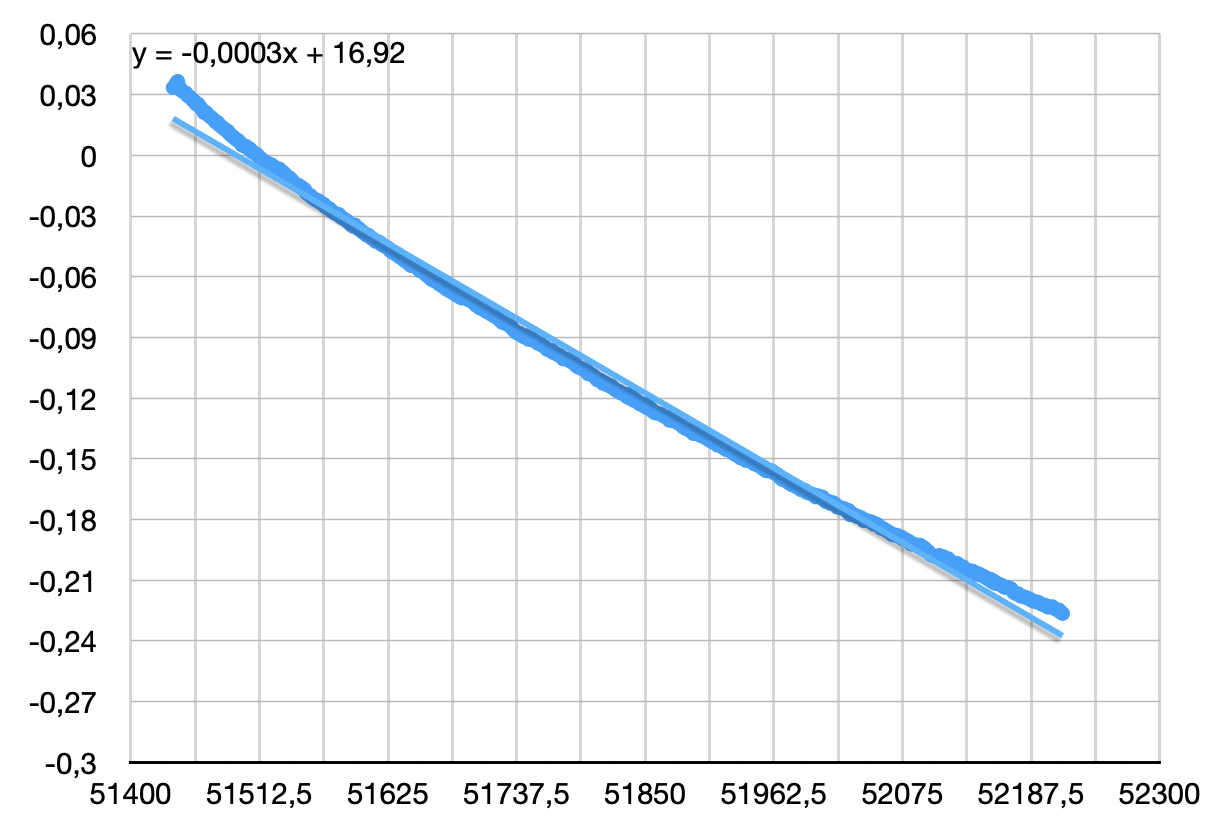
\includegraphics[width = 0.9\linewidth]{down_empty.png}
    \label{fig:d_empty}
    \caption{$T_{cool}(t)$ для пустого каллориметра}
\end{figure}
\begin{figure}
    \centering
    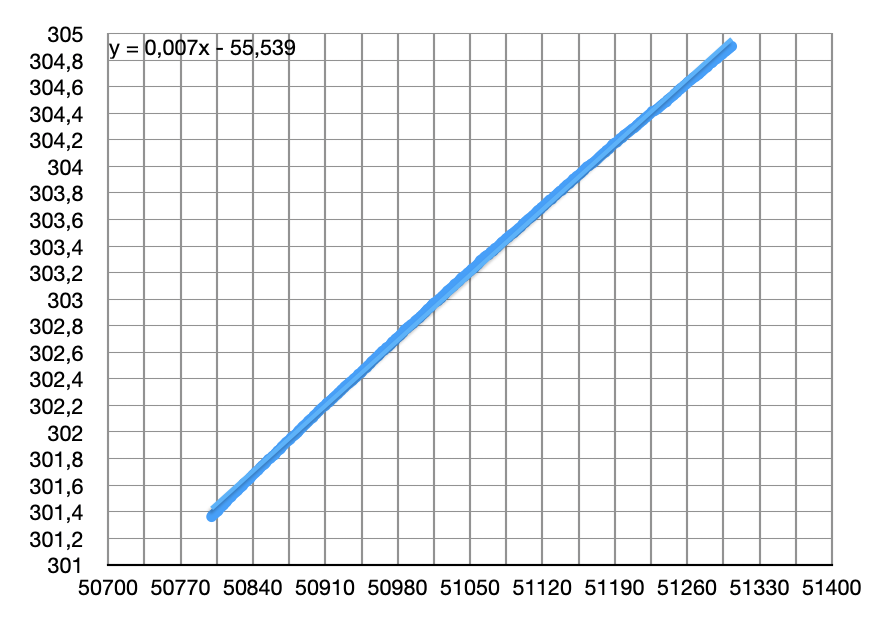
\includegraphics[width = \linewidth]{up_empty.png}
    \label{fig:u_empty}
    \caption{$T_{heat}(t)$ для пустого каллориметра}
\end{figure}
\begin{figure}
    \centering
    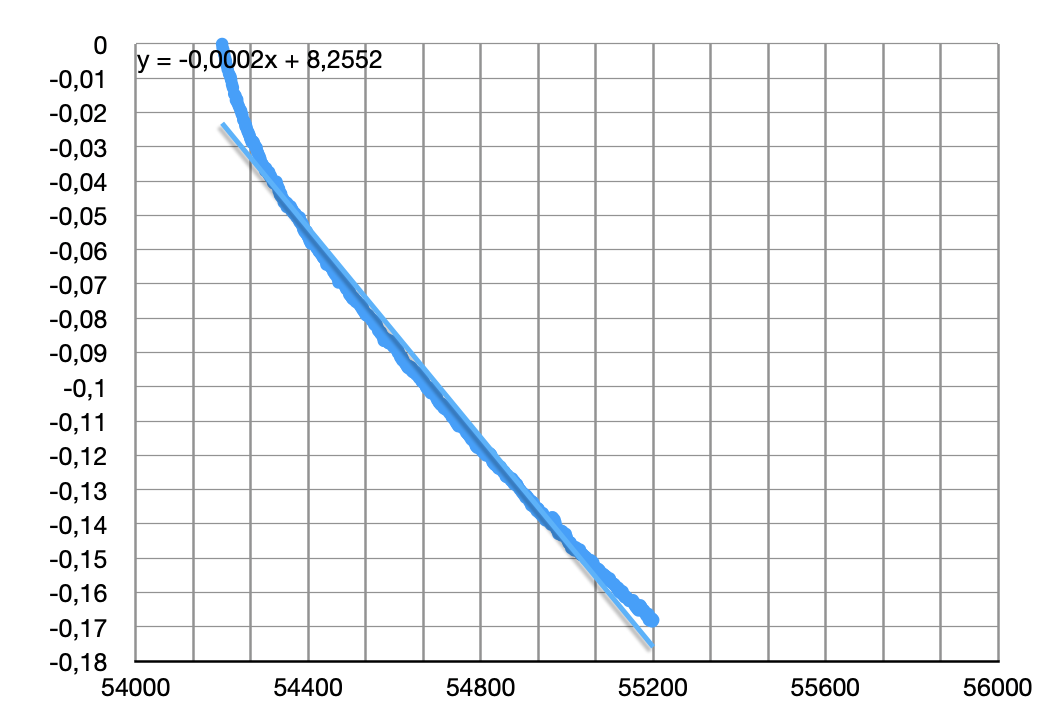
\includegraphics[width = 0.9\linewidth]{down_iron.png}
    \label{fig:d_iron}
    \caption{$T_{cool}(t)$ для железа}
\end{figure}
\begin{figure}
    \centering
    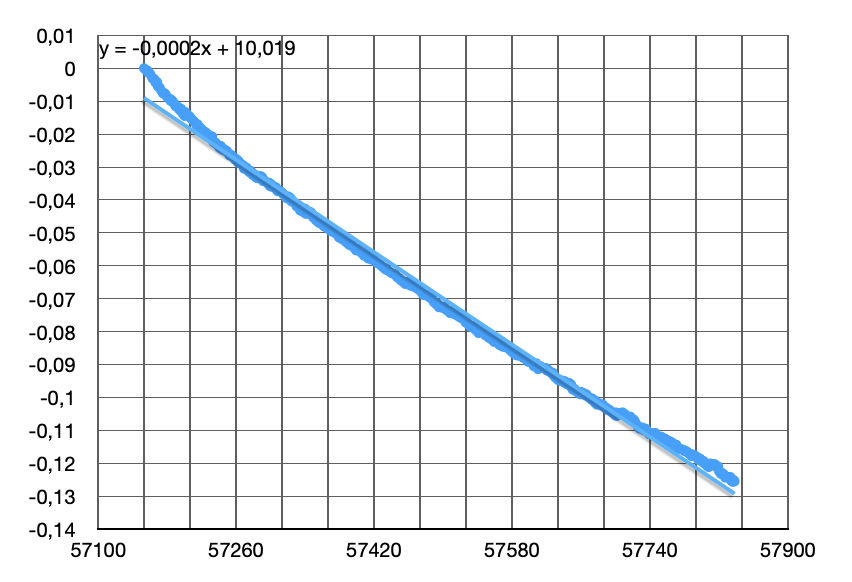
\includegraphics[width = 0.9\linewidth]{down_copper.png}
    \label{fig:d_copper}
    \caption{$T_{cool}(t)$ для меди}
\end{figure}
\begin{figure}
    \centering
    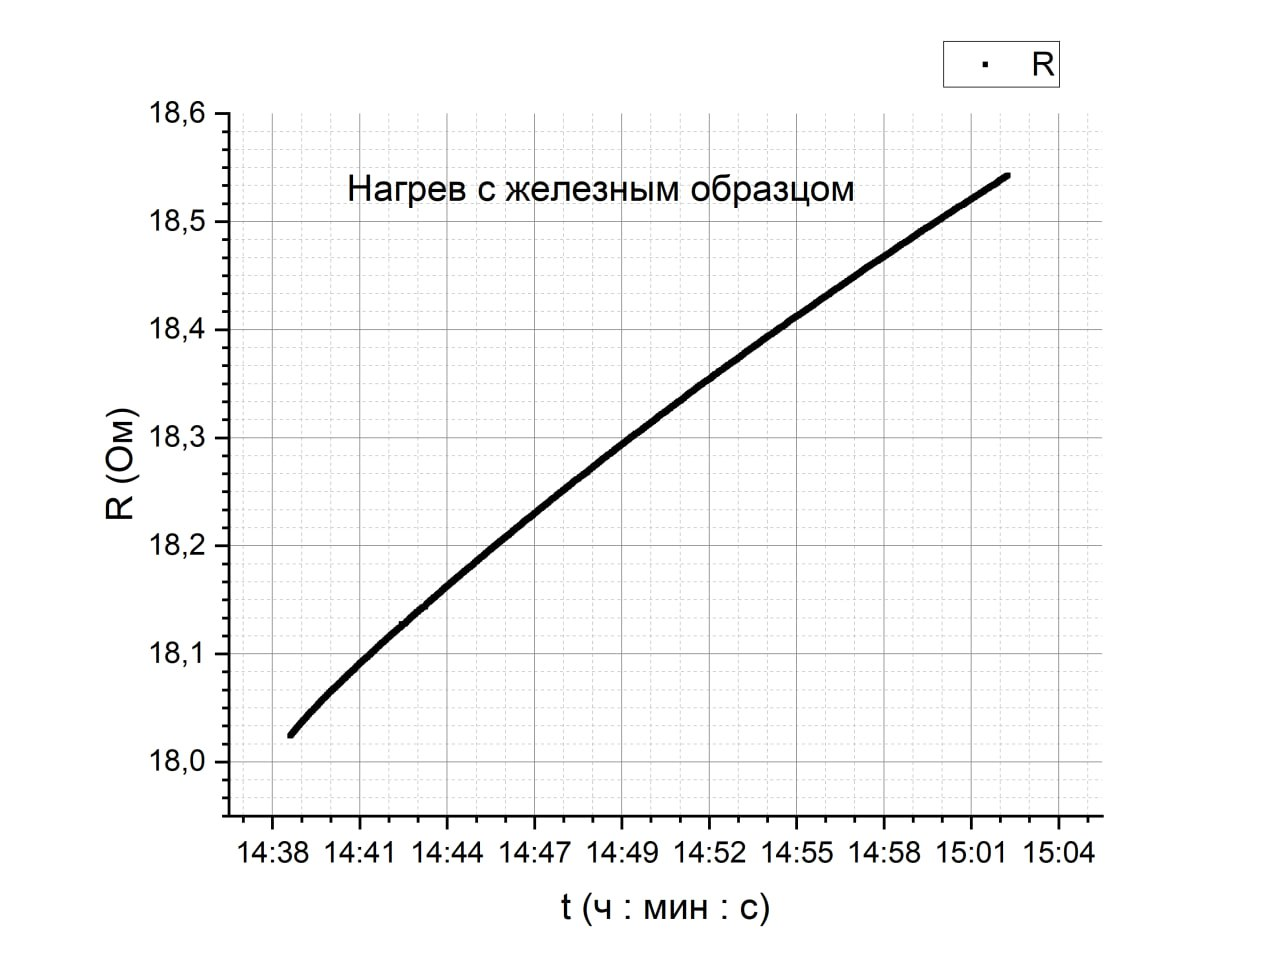
\includegraphics[width = 0.9\linewidth]{up_iron.jpg}
    \label{fig:u_iron}
    \caption{$T_{heat}(t)$ для железа}
\end{figure}
\begin{figure}
    \centering
    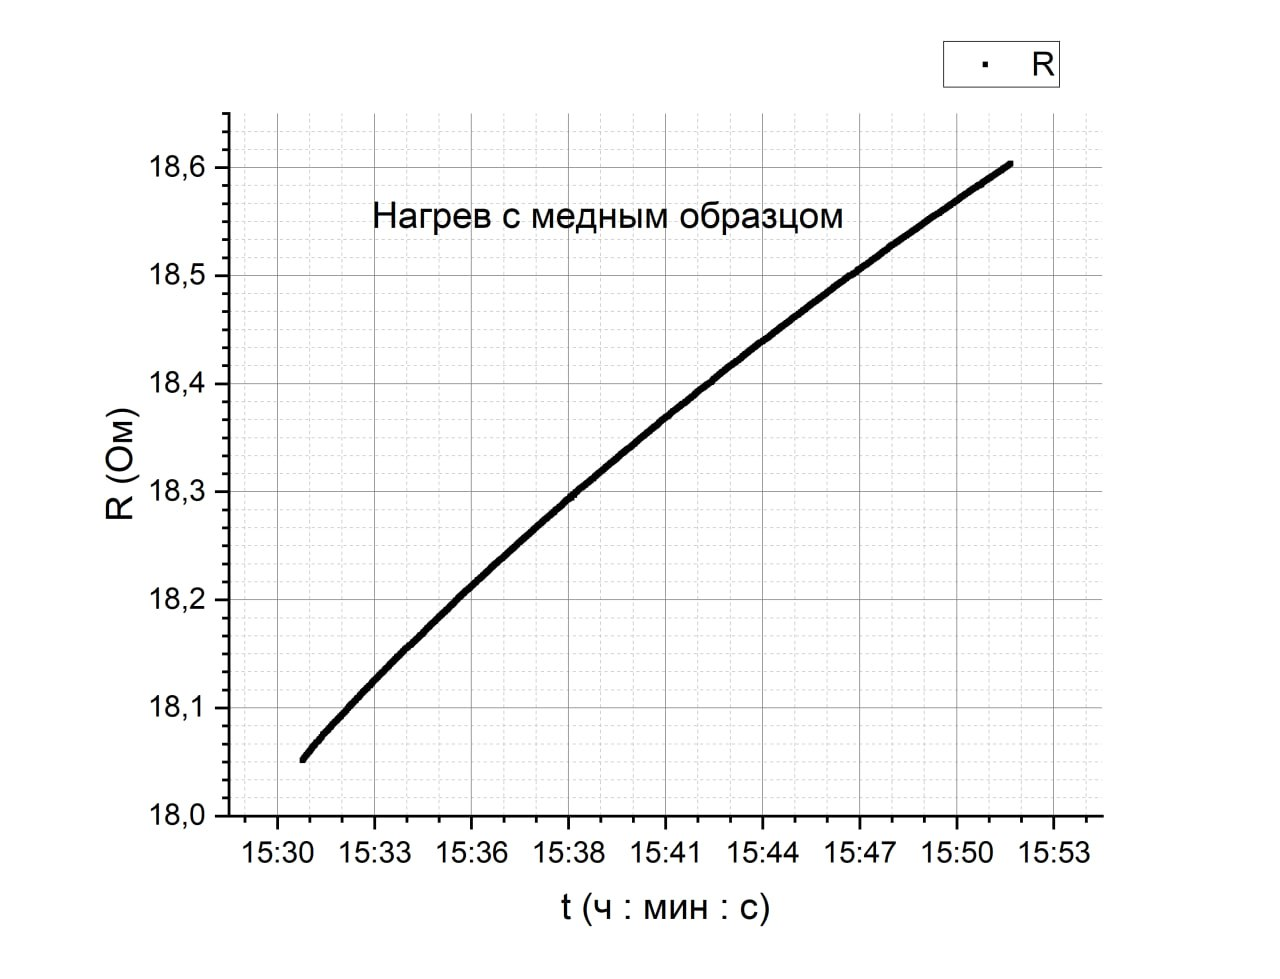
\includegraphics[width = 0.9\linewidth]{up_copper.jpg}
    \label{fig:u_copper}
    \caption{$T_{heat}(t)$ для меди}
\end{figure}
\include{matlab}
\end{document}
